\scriptsize
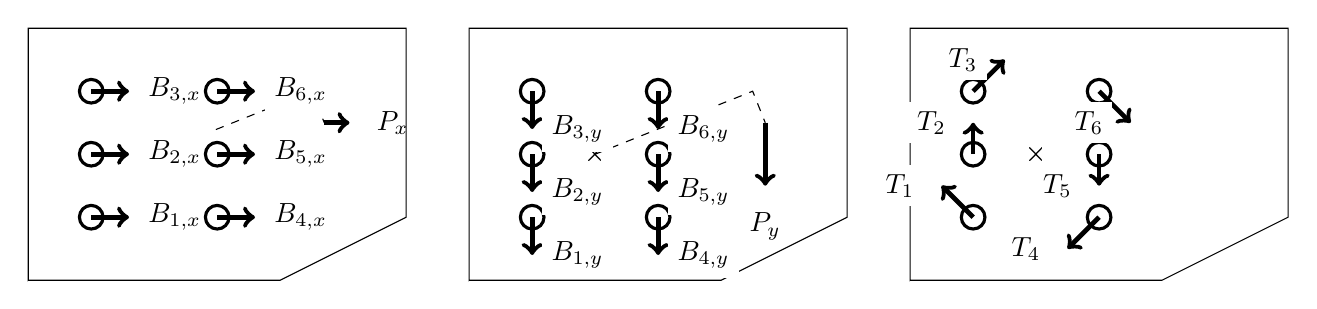
\begin{tikzpicture}[scale=.8]
\draw(-1,-1)--++(4,0)--++(2,1)--++(0,3)-|cycle;
\draw(1,1)node{\texttimes};
\draw[dashed](1,1)--++(2.5,1)--++(.2,-.5)coordinate(A);
\draw[->,line width=.6mm](A)--++(.4,0)node[right=2mm]{$P_x$};
\foreach\x in{0,2}{\foreach\y[evaluate=\y as \z using int(1+\y+1.5*\x)]in{0,1,2}{
\node[circle,inner sep=0pt,minimum size=3mm,line width=.4mm,draw]at(\x,\y){};
\draw[->,line width=.6mm](\x,\y)--++(.6,0)node[right=1mm,fill=white]{$B_{\z,x}$};}}
\begin{scope}[xshift=7cm]
\draw(-1,-1)--++(4,0)--++(2,1)--++(0,3)-|cycle;
\draw(1,1)node{\texttimes};
\draw[dashed](1,1)--++(2.5,1)--++(.2,-.5)coordinate(A);
\draw[->,line width=.6mm](A)--++(0,-1)node[below=2mm]{$P_y$};
\foreach\x in{0,2}{\foreach\y[evaluate=\y as \z using int(1+\y+1.5*\x)]in{0,1,2}{
\node[circle,inner sep=0pt,minimum size=3mm,line width=.4mm,draw]at(\x,\y){};
\draw[->,line width=.6mm](\x,\y)--++(0,-.6)node[right=1mm,fill=white]{$B_{\z,y}$};}}
\end{scope}
\begin{scope}[xshift=14cm]
\draw(-1,-1)--++(4,0)--++(2,1)--++(0,3)-|cycle;
\draw(1,1)node{\texttimes};
\setstructmech{convention=direction}
\NodalForce{1,1}[N][N][-Pe]
\foreach\x in{0,2}{\foreach\y[evaluate=\y as \z using int(1+\y+1.5*\x)]in{0,1,2}{\node[circle,inner sep=0pt,minimum size=3mm,line width=.4mm,draw]at(\x,\y){};}}
\draw[->,line width=.6mm](0,0)--++(-.5,.5)node[fill=white,left=2mm]{$T_1$};
\draw[->,line width=.6mm](0,1)--++(0,.5)node[fill=white,left=2mm]{$T_2$};
\draw[->,line width=.6mm](0,2)--++(.5,.5)node[fill=white,left=2mm]{$T_3$};
\draw[->,line width=.6mm](2,0)--++(-.5,-.5)node[fill=white,left=2mm]{$T_4$};
\draw[->,line width=.6mm](2,1)--++(0,-.5)node[fill=white,left=2mm]{$T_5$};
\draw[->,line width=.6mm](2,2)--++(.5,-.5)node[fill=white,left=2mm]{$T_6$};
\end{scope}
\end{tikzpicture}